\chapter{The Powered Descent Guidance Problem}
\label{mathchapter}



\subsection{Dynamics}
In our formulation, the vehicle is treated as a rigid body. We assume that aerodynamic forces are negligible but that the body is subject to planetary gravitation $\mathbf{g}_I$. The algorithm as presented in \cite{6dofsucc} has the vehicle actuated by a single gimbaled thruster at the bottom of the vehicle. This engine has feasible thrust magnitude and efficiency, as well as standard gimbal range for agile vehicles. Modifications can be made here to include other actuators in the dynamics. I could have adapted my own actuator dynamics here, but to save time I have implemented the original algorithm.

We also capture mass depletion dynamics, proportional to the magnitude of the thrust generated by the engine. For tractability, we assume that the inertia matrix and the position of the center-of-mass is constant throughout the trajectory. We use the constant $\alpha_{\dot{m}}$, a function of the specific impulse, as the mass depletion parameter. Therefore we have that
\begin{align}
& \alpha_{\dot{m}} = \frac{1}{I_{sp} g_0} \\
& \dot{m}(t) = -\alpha_{\dot{m}} \left\lVert \mathbf{T}_B{t} \right\rVert _2
\end{align}

We will express the translational dynamics and forces acting on the vehicle in the inertially fixed frame. They are as follows:

\begin{align}
& \dot{\mathbf{r}}_I(t) = \mathbf{v}_I(t) \\
& \dot{\mathbf{v}}_I(t) = \frac{\mathbf{F}_I}{m(t)} + \mathbf{g}_I
\end{align}

The attitude formalism used in the paper are Euler parameters, or quaternions. They are used to denote the attitude of the vehicle between the $\mathcal{F}_B$ and $\mathcal{F}_I$ frames, $q_{B/I}(t)$ on the unit sphere. We use the angle-axis form of the quaternion, noted here:

\begin{align}
q_{B/I}(t) \triangleq 
	\begin{bmatrix}
	\cos(\phi/2) \\ \hat{n}\sin(\phi/2)
	\end{bmatrix}
	= 
	\begin{bmatrix}
	q_1 \quad q_2 \quad q_3 \quad q_4
	\end{bmatrix}^T
\end{align}

The $\hat{n} \in \mathcal{R}^3$ vector is the euler vector in which the single angle $\phi$ displaces the attitude about. In our derivation we will also need the direction cosine matrix produced by this quaternion. DCMs are part of the $SO(3)$ group with properties that its determinant is 1 and can be transposed/inverted for the reverse mapping. They can be multiplied to encode multiple rotations. The mapping from inertial to body frame is the following:

\begin{align}
C_{B/I}={\begin{bmatrix}1-2(q_{2}^{2}+q_{3}^{2})&2(q_{1}q_{2}-q_{0}q_{3})&2(q_{0}q_{2}+q_{1}q_{3})\\2(q_{1}q_{2}+q_{0}q_{3})&1-2(q_{1}^{2}+q_{3}^{2})&2(q_{2}q_{3}-q_{0}q_{1})\\2(q_{1}q_{3}-q_{0}q_{2})&2(q_{0}q_{1}+q_{2}q_{3})&1-2(q_{1}^{2}+q_{2}^{2})\end{bmatrix}}
\end{align}

In our attitude dynamics, we will use $\bm{\omega}_B(t) \in \mathcal{R}^3$ to denote the angular velocity vector of the vehicle in the $\mathcal{F}_B$ frame with respect to $\mathcal{F}_I$. The torque acting on the vehicle is written as $\mathbf{M}_B(t) \in \mathcal{R}^3$ in the body frame. We also use the $\left[\mathbf{r}^\times \right]$ operator to denote the skew symmetric form of the vector $\mathbf{r}$. The inertia tensor instantiated in $\mathcal{F}_B$ is written as $J_B \in \mathcal{R}^{3\times 3}$.

Given that we have chosen quaternions as our formalism, we must understand the kinematics as such:

\begin{align}
 & \dot{q}_{B/I}(t) = \frac{1}{2} B(\bm{\omega_B}(t)) q_{B/I}(t)
\end{align}

where the matrix $B(\bm{\omega_B}(t))$ is defined as 
\begin{align}
& B(\bm{\omega_B}(t)) = 
	\begin{bmatrix}
	0 & -\omega_1 & -\omega_2 & -\omega_3\\ 
	\omega_1 & 0 & \omega_3 & -\omega_2 \\
	\omega_2 & -\omega_3 & 0 & \omega_1 \\
	\omega_3 & \omega_2 & -\omega_1  & 0  \\
	\end{bmatrix}
\end{align}

We can also derive the simplified angular dynamics as the following
\begin{align}
& J_B \dot{\bm{\omega}}_B(t) = -\left[\bm{\omega}_B ^ \times\right] J_B \bm{\omega}_B + \mathbf{M}_B(t)
\end{align}
With the torque applied to the spacecraft.


\subsection{Constraints and Boundary Conditions}
We must now state the constraints and boundary values for the problem required by the optimization.
We know that we can never use more fuel than we have, therefore the convex constraint is 
\begin{align}
& m(t) \geq m_{dry}
\end{align}

Additionally we want to apply a glide slope constraint in the case that our vehicle has terrain relative navigation sensors. We form the convex constraint using the angle $\gamma_{gs}$:
\begin{align}
& \mathbf{e}_1 \cdot \mathbf{r}_I(t) \geq \tan(\gamma_{gs}) \left\lVert \left[\mathbf{e}_2 \quad \mathbf{e}_3\right]^T \mathbf{r}_I(t) \right\lVert_2
\end{align}
This effectively draws an upward facing cone slope that the vehicle must not penetrate. This type of convex constraint can also be useful in avoiding rocky terrain and enforcing a landing from directly above an area, minimizing lateral movement close to the ground.
The author also included that the vehicle must avoid excessive tilt angles such that it stays relatively upright throughout the trajectory, we can constrain a portion of the direction cosine matrix as such:
\begin{align}
& \cos(\theta_{max}) \leq 1-2(q_{2}^{2}+q_{3}^{2})
\end{align}

Along the same line of thought, we can constrain the angular rate using convex constraints as well:
\begin{align}
& \left \lVert \bm{\omega}_B(t) \right \lVert_2 \leq \omega_{max}
\end{align}

Finally we must encode that the commanded thrust vector needs to be constrained between two magnitudes, which is appropriate. We assume that the engine cannot be re-lit during operation (commonly becoming a bad assumption to make). We also know that there is some limit to the amount of gimbal angle we can perform $\delta_{max}$.
\begin{align}
& 0 < T_{min} \leq \left \lVert \bm{T}_B(t) \right \lVert_2 \leq T_{max} \\
& \cos(\delta_{max}) \left \lVert \bm{T}_B(t) \right \lVert_2 \leq \bm{e}_1 \cdot \bm{T}_B(t)
\end{align}

We see that the upper thrust bound is clearly convex but the lower bound creates a non-convex constraint. Because of the range of  $\delta_{max}$ turns out to be convex.

For the powered descent guidance problem, the boundary conditions are trivial to identify. The initial mass, position, velocity, attitude, and angular rates are given by the navigation subsystem at the moment in time. We assume the dry mass is known and that and estimate of the wet mass can be backed out. The terminal position is the landing site. The terminal translational and angular velocities can be zero, with the terminal attitude in the upright position. The final mass should be free. The initial thrust vector should be free, while the terminal vector should be along the vehicle up, X-axis. The author intends on the initial attitude being free, which can free up the optimization for shorter final times.




\subsection{Continuous Time Problem}
Putting this all together we can pose the continuous time optimization problem. In this form, it is non-convex and requires significant conditioning to work into the convex framework. As stated, the objective is to minimize the time-of-flight required to get to the terminal conditions subject to the aforementioned constraints, dynamics, and boundary conditions. We leave the commanded thrust, gimbal angles, and final time free. It is as follows:
\clearpage

\begin{mdframed}
\textbf{Problem 1: Continuous Time Non-Convex Free-Final-Time}

\underline{Cost Function:}
\begin{equation*}
\min_{\mathbf{T}_B, t_f} t_f
\end{equation*}

\underline{Boundary Conditions:}  
\begin{align*}
& m(0) = m_{wet} \quad \mathbf{r}_I(0) = \mathbf{r}_i \quad \mathbf{v}_I(0) = \mathbf{v}_i \quad \quad \quad{q}_{B/I}(0) = {q}_{B/I _{i}} \quad \bm{\omega}_B(0) = \bm{\omega}_{B _{i}} \\
& \mathbf{r}_I(t_f) = \mathbf{0} \quad \quad \mathbf{v}_I(t_f) = \mathbf{0} \quad {q}_{B/I}(t_f) = {q}_{B/I _ {f}} \quad \bm{\omega}_B(t_f) = \mathbf{0} \\
& \mathbf{e}_2 \cdot \mathbf{T}_B(t_f) = \mathbf{e}_3 \cdot \mathbf{T}_B(t_f) = 0
\end{align*}

\underline{Dynamics:}  
\begin{align*}
& \dot{m}(t) = -\alpha_{\dot{m}} \left\lVert \mathbf{T}_B{t} \right\rVert _2 \\
& \dot{\mathbf{r}}_I(t) = \mathbf{v}_I(t) \\
& \dot{\mathbf{v}}_I(t) = \frac{C_{I/B}(t)\mathbf{T}_B(t)}{m(t)} + \mathbf{g}_I \\
 & \dot{q}_{B/I}(t) = \frac{1}{2} B(\bm{\omega_B}(t)) q_{B/I}(t) \\
& J_B \dot{\bm{\omega}}_B(t) = -\left[\bm{\omega}_B ^ \times\right] J_B \bm{\omega}_B + \left[r_{com}^\times \right]\mathbf{T}_B(t)
\end{align*}

\underline{State Constraints:}  
\begin{align*}
& m(t) \geq m_{dry} \\
& \mathbf{e}_1 \cdot \mathbf{r}_I(t) \geq \tan(\gamma_{gs}) \left\lVert \left[\mathbf{e}_2 \quad \mathbf{e}_3\right]^T \mathbf{r}_I(t) \right\lVert_2 \\
& \cos(\theta_{max}) \leq 1-2(q_{2}^{2}+q_{3}^{2}) \\
& \left \lVert \bm{\omega}_B(t) \right \lVert_2 \leq \omega_{max}
\end{align*}

\underline{Control Constraints:}  
\begin{align*}
& 0 < T_{min} \leq \left \lVert \bm{T}_B(t) \right \lVert_2 \leq T_{max} \\
& \cos(\delta_{max}) \left \lVert \bm{T}_B(t) \right \lVert_2 \leq \bm{e}_1 \cdot \bm{T}_B(t)
\end{align*}

\end{mdframed}




\section{Convex Form}
Now we shall derive the convex form of Problem 1. We will convert the non-convex continuous free-final-time problem to a convex fixed-final-time problem. This will be a second order cone sub-problem. We will solve this sub-problem repeatedly to convergence or "successively." This successive process turns each subproblem into a larger free-final-time algorithm.

\subsection{Linearization}
Let us define the state vector $\mathbf{x}(t) \in \mathcal{R}^{14\times 1}$ and our control vector $\mathbf{u}(t) \in \mathcal{R}^{3\times 1}$:
\begin{align}
& \mathbf{x}(t) \triangleq 
	\begin{bmatrix}
	m(t) & \mathbf{r}_I^T(t) & \mathbf{v}_I^T(t) & q_{B/I}^T(t) & \bm{\omega}_B^T(t)   
	\end{bmatrix}^T \\
& \mathbf{u}(t) \triangleq \mathbf{T}_B(t)  
\end{align}
Therefore we can express the nonlinear dynamics in the following form
\begin{align}
& \frac{d}{dt}\mathbf{x}(t) = f(\mathbf{x}(t), \mathbf{u}(t)) =  
	\begin{bmatrix}
	\dot{m(t)} & \dot{\mathbf{r}}_I^T(t) & \dot{\mathbf{v}}_I^T(t) & \dot{q}_{B/I}^T(t) & \dot{\bm{\omega}}_B^T(t)  
	\end{bmatrix}^T
\end{align}

In order to make the problem free-final-time, we must manipulate the how time works. We are going to replace $t$ with a normalized trajectory time $\tau \in \left[0,1\right]$. We apply the chain run:


\begin{align}
& \frac{d}{dt}\mathbf{x}(t) = \frac{d\tau}{dt} \frac{d}{d\tau}\mathbf{t}(t)
\end{align}

And we can translate between the two by using the dilation coefficient $\sigma$ which is defined
\begin{align}
& \sigma \triangleq \Big(\frac{d\tau}{dt}\Big)^{-1}
\end{align}

This $\sigma$ will become a variable in the convex subproblem that acts as the non-dimensionalized final time. It is a scaling factor that translates between real work differential time and the normalized version used for our algorithm. We can now write the nonlinear dynamics to take advantage of this normalized time:

\begin{align}
& \mathbf{x}^\prime(\tau) \triangleq \frac{d}{d\tau}\mathbf{x}(\tau) = \sigma f(\mathbf{x}(\tau), \mathbf{u}(\tau))
\end{align}

We can fit the nonlinear dynamics from problem 1 into a linear framework by performing a first-order Taylor approximation about a reference state, input, and dilation coefficient $(\hat{\mathbf{x}}, \hat{\mathbf{u}}, \hat{\sigma})$. Therefore we can represent the system using normalized time:

\begin{align}
& \mathbf{x}^\prime(\tau) = \hat{\sigma}\frac{\partial}{\partial x} f(x,u) \bigg\rvert_{\hat{x},\hat{u}}(x(\tau)-\hat{x}(\tau)) + \hat{\sigma}\frac{\partial}{\partial u} f(x,u) \bigg\rvert_{\hat{x},\hat{u}}(u(\tau)-\hat{u}(\tau)) + \sigma f(\hat{x}(\tau),\hat{u}(\tau)) \\
& \mathbf{x}^\prime(\tau) = A(\tau)\mathbf{x(\tau)} + B(\tau)\mathbf{u(\tau)} + \Sigma(\tau)\sigma + \mathbf{z}(\tau)
\end{align}

We can break the Taylor expansion into matrices to make things simpler later on:
\begin{align}
& A(\tau) \triangleq \hat{\sigma} \frac{\partial}{\partial x} f(x,u) \bigg\rvert_{\hat{x},\hat{u}} \\
& B(\tau) \triangleq \hat{\sigma} \frac{\partial}{\partial u} f(x,u) \bigg\rvert_{\hat{x},\hat{u}} \\
& \Sigma(\tau) \triangleq f(\hat{x}(\tau),\hat{u}(\tau)) \\
& \mathbf{z}(\tau) \triangleq -A(\tau)\hat(x)(\tau) - B(\tau)\hat{u}(\tau)
\end{align}

With this done, we tackle the only source of non-convexity: the non-zero lower bound to our actuator thrust. With a Taylor series approximation we can say that $T_{min} \leq B_g(\tau)\mathbf(u)(\tau)$ for which $B_g(\tau) \triangleq \frac{\mathbf{\hat{u}}^T(\tau)}{\left\lVert \mathbf{\hat{u}} \right \lVert_2}$.



\subsection{Discretization Scheme}
This is where things get hairy. We need to "cast" the problem into a finite dimensional optimization problem where the trajectory is discretized into $K$ evenly separated points with respect to the normalized trajectory time $\tau$. Let us define the set $\mathcal{K}\triangleq \{0,1,\cdots, K-1\}$ with which many of the parameter arrays will have the same dimensions.

Given that the trajectory time is normalized on the interval $\tau \in [0,1 ]$, we must define the discrete time step at point $k$ as such

\begin{align}
& \tau_k \triangleq \frac{k}{K-1}, \quad \forall k \in \mathcal{K}
\end{align}

To help with numerical feasibility issues, we employ a first-order-hold linear scaling on the applied controls for each time step. Over the interval $\tau \in [\tau_k, \tau_{k+1}]$, we must express $\mathbf{u}(\tau)$ in terms of the $\mathbf{u}_k$
 and $\mathbf{u}_{k+1}$:

 \begin{align}
& \mathbf{u}(\tau) \triangleq \alpha_k(\tau) \mathbf{u}_k + \beta(\tau) \mathbf{u}_{k+1} \\ 
& \alpha_k(\tau) = \frac{d\tau - \tau}{d\tau} \\
& \beta_k(\tau) = \frac{\tau}{d\tau} \\
& d\tau = \frac{1}{K-1}
\end{align}

I have shown these differently than the author for simplicity.

We can then use a state transition matrix $\Phi(\tau_{k+1},\tau_k)$ to translate the system from $k$ to $k+1$ with no input. This matrix follows these dynamics:
\begin{align}
& \frac{d}{d\tau} \Phi(\tau,\tau_k) = A(\tau) \Phi(\tau,\tau_k) \quad \forall k \in \mathcal{K}
\end{align}

Using our previous expressions, we can now discretize the dynamics such that each matrix, at each time step requires a short integration:
 \begin{align}
& \mathbf{x}_{k+1} = \bar{A}_k\mathbf{x_k} + \bar{B}_k\mathbf{u_k} + \bar{C}\mathbf{u_{k+1}} + \bar{\Sigma}_k\sigma + \bar{\mathbf{z}}_k  \\
& \bar{A}_k \triangleq  \Phi(\tau_{k+1},\tau_k)\\
& \bar{B}_k \triangleq \int_{\tau_k}^{\tau_{k+1}} \alpha_k(\xi) \Phi(\tau_{k+1},\xi) B(\xi) d\xi\\
& \bar{C}_k \triangleq \int_{\tau_k}^{\tau_{k+1}} \beta_k(\xi) \Phi(\tau_{k+1},\xi) B(\xi)  d\xi\\
& \bar{\Sigma}_k \triangleq \int_{\tau_k}^{\tau_{k+1}} \Phi(\tau_{k+1},\xi) \Sigma(\xi) d\xi\\
& \bar{\mathbf{z}}_k \triangleq \int_{\tau_k}^{\tau_{k+1}} \Phi(\tau_{k+1},\xi) \mathbf{z}(\xi) d\xi\\
\end{align}

The other boundary, state, and control constraints are already convex and just need to be instantiated for all time or at initial/terminal $\tau$.


\subsection{Successive Form, Trust Regions and Relaxations}
In order to solve a non-convex problem, we iteratively solve a sequence of related convex subproblems. However, before we can reach a concluding framework, we must consider trust regions and dynamic relaxations. In order to make sure that this successive framework stays bounded and feasible through this convergence process, we must bound the divergence of state and inputs from one iteration to another. Unbounded problems can arise from constraints that admit an unbounded cost. To mitigate this issue, we augment the cost function with soft trust regions about the previous iterate's information. Let us define these deviations at iteration $i$ as such:
\begin{align}
& \delta \mathbf{x}_k^i \triangleq \mathbf{x}_k^i - \mathbf{x}_k^{i-1} \\
& \delta \mathbf{u}_k^i \triangleq \mathbf{u}_k^i - \mathbf{u}_k^{i-1}, \quad \forall k \in \mathcal{K}\\
& \delta \sigma^i \triangleq \sigma^i - \sigma^{i-1}
\end{align}

We can then fabricate the following constraints with $\bm{\bar{\Delta}}^i \in \mathcal{R}^K$ and $\Delta_\sigma^i \in \mathcal{R}$
\begin{align}
& \delta \mathbf{x}_k^i \cdot \delta \mathbf{x}_k^i + \delta \mathbf{u}_k^i \cdot \delta \mathbf{u}_k^i \leq \mathbf{e}_k \cdot \bm{\bar{\Delta}}^i \\
& \delta \sigma^i \cdot \delta \sigma^i \leq \Delta_\sigma^i
\end{align}

We can now append $w_\Delta^i \norm{{\bar{\Delta}}^i} + w_{\Delta_\sigma}\norm{\Delta_\sigma^i}$ to the cost function to attempt to minimize input, state, and final time deviations and keeping their deviation bounded via constraint, where $w_\Delta^i$ and $w_{\Delta_\sigma}$ are weighting scalars.
Here the author makes an important note. Given that the trust regions are centered about previous points $(\mathbf{x}_{k}^{i-1},\mathbf{u}_{k}^{i-1},\sigma^{i-1})$, we must evaluate the Jacobian about the nonlinear trajectory beginning at $\mathbf{x}_{k}^{i-1}$. We can then use the zero-order-hold input vector $\mathbf{u}(\tau)$. Doing this $\forall k \in \mathcal{K}$ defines the linearization path $(\hat{\mathbf{x}}, \hat{\mathbf{u}}, \hat{\sigma})$.

Finally we must speak to dynamic relaxation. "Artificial Infeasibility" is  encountered during the convergence process when the linearization becomes infeasible. For example, if the dynamics are linearized about unrealistic conditions, it because dynamically inconsistent. It will not produce a feasible solution. This is encountered during the first couple iterations of a successive convexification due to poor initial trajectory or time-of-flight estimation. To get rid of this issue, we employ dynamic relaxation, where a slack variable is added to the dynamics in order to "make room" for the iteration to proceed. However, you can guess that this will inevitably be something we try to minimize in the cost function in order to make sure that our final trajectories are as dynamically consistent as possible. Therefore, we must now write our dynamics as follows: 

\begin{align}
& \mathbf{x}_{k+1}^i = \bar{A}_k^i\mathbf{x_k}^i + \bar{B}_k^i\mathbf{u_k}^i + \bar{C}^i\mathbf{u_{k+1}}^i + \bar{\Sigma}_k^i\sigma^i + \bar{\mathbf{z}}^i_k + \bm{\nu}_k^i
\end{align}

Because we are going to use this in our cost function as a norm, we shall concatenate the time history of the slack variable as

\begin{align}
\bar{\bm{\nu}}^i = 
	\begin{bmatrix}
	{\bm{\nu}_0^i}^T & \cdots & {\bm{\nu}^i_{K-2}}^T 
	\end{bmatrix}^T
\end{align}

And of course we augment the cost function again with $w_v \norm{\bar{\bm{\nu}}^i}_1$. As the iteration continues, this value is minimized as the solution becomes more dynamically feasible. Therefore, the magnitude of this norm is indicative of a final solution in the successive iteration process.

\clearpage
\subsubsection{Convex Sub-Problem}
We can now put all of the components together and form the convex version of the continuous problem, but with fixed final time.

\begin{mdframed}
\textbf{Problem 2: Discretized Convex Fixed-Final-Time Sub-Problem ($i^{th}$ iteration)}
\underline{Cost Function:}
\begin{equation*}
\min_{\sigma^i, \mathbf{u}_k^i} \quad \sigma^i + w_\Delta^i \left\lVert \bar{\Delta}^i \right\lVert_2 + w_{\Delta_\sigma}\left\lVert\Delta_\sigma^i\right\lVert_1 + w_v \left\lVert\bar{\bm{\nu}}^i\right\lVert_1
\end{equation*}

\underline{Boundary Conditions:}  
\begin{align*}
& m_0 = m_{wet} \quad \mathbf{r}_{I_0} = \mathbf{r}_i \quad \mathbf{v}_{I_0} = \mathbf{v}_i \quad \quad \quad{q}_{B/I_0} = {q}_{B/I _{i}} \quad \bm{\omega}_B(0) = \bm{\omega}_{B _{i}} \\
& \mathbf{r}_{I_K} = \mathbf{0} \quad \quad \mathbf{v}_{I_K} = \mathbf{0} \quad {q}_{B/I _K} = {q}_{B/I _ {f}} \quad \bm{\omega}_{B_K} = \mathbf{0} \\
& \mathbf{e}_2 \cdot \mathbf{T}_{B_K}= \mathbf{e}_3 \cdot \mathbf{T}_{B_K}= 0
\end{align*}

\underline{Dynamics:}  
\begin{align*}
& \mathbf{x}_{k+1}^i = \bar{A}_k^i\mathbf{x_k}^i + \bar{B}_k^i\mathbf{u_k}^i + \bar{C}^i\mathbf{u_{k+1}}^i + \bar{\Sigma}_k^i\sigma^i + \bar{\mathbf{z}}^i_k + \bm{\nu}_k^i
\end{align*}

\underline{State Constraints:}  
\begin{align*}
& m_k \geq m_{dry} \\
& \mathbf{e}_1 \cdot \mathbf{r}_{I_k} \geq \tan(\gamma_{gs}) \left\lVert \left[\mathbf{e}_2 \quad \mathbf{e}_3\right]^T \mathbf{r}_{I_k} \right\lVert_2 \\
& \cos(\theta_{max}) \leq 1-2(q_{2_k}^{2}+q_{3_k}^{2}) \\
& \left \lVert \bm{\omega}_{B_k} \right \lVert_2 \leq \omega_{max}
\end{align*}

\underline{Control Constraints:}  
\begin{align*}
& T_{min} \leq B_g(\tau_k)\mathbf{u}_k^i \\
& \left \lVert \mathbf{u}_k^i \right \lVert_2 \leq T_{max} \\
& \cos(\delta_{max}) \left \lVert \mathbf{u}_k^i \right \lVert_2 \leq \bm{e}_1 \cdot \mathbf{u}_k
\end{align*}

\underline{Trust Regions:}  
\begin{align*}
& \delta \mathbf{x}_k^i \cdot \delta \mathbf{x}_k^i + \delta \mathbf{u}_k^i \cdot \delta \mathbf{u}_k^i \leq \mathbf{e}_k \cdot \bm{\bar{\Delta}}^i \\
& \delta \sigma^i \cdot \delta \sigma^i \leq \Delta_\sigma^i
\end{align*}

\end{mdframed}



\clearpage
\section{Algorithm}
The goal is for the successive convexification algorithm to continue iterating until $\Delta_{tol}$ and $\nu_{tol}$ are met. These are defined by the magnitude of each vector.

\begin{algorithm}
\caption{Successive Convexification}\label{Successive}
\begin{algorithmic}[1]
\Procedure{SCVX}{$x_{ref},\sigma_{ref}$}
\State Generate initial trajectory by linearly spanning from initial condition to terminal conditions on each state
\While{$ ||{\Delta}|| \geq \Delta_{tol} \quad \&\& \quad ||{\nu}|| \geq \nu_{tol} $}
\State Compute $\bar{A}_k^{i-1}, \bar{B}_k^{i-1}, \bar{C}_k^{i-1}, \bar{\Sigma}_k^{i-1}, \bar{z}_k^{i-1}$ from $\mathbf{x}_k^{i-1}, \mathbf{u}_k^{i-1}, \sigma^{i-1}$
\State Solve Problem 2 using $\mathbf{x}_k^{i-1}, \mathbf{u}_k^{i-1}, \sigma^{i-1}, \bar{A}_k^{i-1}, \bar{B}_k^{i-1}, \bar{C}_k^{i-1}, \bar{\Sigma}_k^{i-1}, \bar{z}_k^{i-1}$
\State Store the newly found $\mathbf{x}_k^{i}, \mathbf{u}_k^{i}, \sigma^{i}$
\State $i++;$
\EndWhile 
\State \textbf{return} $\mathbf{x}, \mathbf{u}$
\EndProcedure
\end{algorithmic}
\end{algorithm}


% \begin{figure}[!htb] 
%   \centering
%   \includegraphics[width=0.5\textwidth]{alg.PNG}
%   \caption{Diagram depicting how the successive convexification loop works. If the tolerance requirements are not met, another iteration is done again to make sure it is producing dynamically feasible sets.}
%   \label{fig:succ}
%  \end{figure}

It turns out that this tool is incredibly powerful. One can modify the dynamics quite a bit, and depending on the robustness of the linearization scheme, this could be used as a generalized tool. The only glaring obstacle is state and actuator constraints. These types of nonconvexities need to be managed carefully.



\section{Dimensionalized Simulation Results}
The initial conditions to this problem must be small for numerical stability. Therefore, you must non-dimensionalize then on entry. Once the problem is solved, you can redimensionalize the solution, as shown in \ref{fig:succ}. I implemented this algorithm in Python, utilizing the CVXPY library with ECOS solver. Below in \ref{table:nonlin} are some parameters I tested for an in-plane maneuver. I used the same constants and weightings as in \cite{6dofsucc}. For this scenario, to redimensionalize, $U_M = 10$kg, $U_L=100$meters, and $U_T = (10)^{1/2}$seconds.

\begin{table}[ht]
\caption{Parameters Used}
\centering 
\begin{tabular}{c c c} 
\hline\hline
Param & Units & Value \\ [0.5ex] 
\hline 
$\mathbf{g}_I$ 		& $U_L/U_T^2$ 	& $-0.981\mathbf{e}_1$ 		\\ 
$\alpha_{\dot{m}}$ 	& - 			& 0.004 							\\
$m_{wet}$ 			& $U_M$ 		& 14		 					\\
$m_{dry}$ 			& $U_M$ 		& 3  						\\
$r_{I_0}$ 			& $U_L$ 		& $(4,4,0)$ 							\\
$v_{I_0}$ 			& $U_L/U_T$	 	& $(-0.1,0,0)$ 							\\
$q_{{BI}_0}$ 		& - 			& $(1,0,0,0)$ 							\\
$\omega_{B_0}$ 		& $rad/U_T$ 			& $(0,0,0)$ 							\\[1ex] 
\hline
\end{tabular}
\label{table:nonlin}
\end{table}


% \begin{figure}[!htbp] 
%   \centering
%   \includegraphics[width=\textwidth]{guidplots.PNG}
%   \caption{Top Left - Planar trajectory plotted in 3D with quivers acting as thrust vector and magnitude indicators. The trajectory looks smooth and dynamically consistent. Top Right - This plot displays the thrust on each axis, the magnitude, and the thrust angle. These look very jagged and non-differentiable. Numerical problems could cause this. Ideally we would like to actuate the engine at lower gimbal rates. Lower Left - The attitudes generated look smooth and dynamically consistent. Lower Right - The mass depletion is shown. It seems to only have consumed 4kg of propellant over the $\sigma=$ 6.474.}
%   \label{fig:guidplots}
%  \end{figure}


\section{Attitude Trajectory Tracking with Cold Gas Thrusters}
This portion of the project was developed for ASEN6010 Advanced Attitude Control. I will now show how control can be done with thrusters at the top of the vehicle. I am using the attitude trajectory generated from the convex optimal problem. I have converted those quaternions into MRPs and switched from the UEN frame to a more common ENU frame. This is to say that +x is in the direction of thruster 2 on figure \ref{fig:thrusters}; +y goes along thruster 1, and thruster 6/8 generate a positive torque about the z-axis axially through the top.

Please note that I did not implement standard Schmitt trigger "bang bang" control here. This probably would have been a more realistic implementation.

% \begin{figure}[!htbp] 
% \centering
% \begin{minipage}{.5\textwidth}
%   \centering
%   \includegraphics[width=.4\linewidth]{vehicle.png}
%   \captionof{figure}{Example vehicle where circles represent cold gas thruster placement, $\mathbf{r}_i$ represents distance to thruster, and $g_t$ represents pointing vector.}
%   \label{fig:vehicle}
% \end{minipage}%
% \begin{minipage}{.5\textwidth}
%   \centering
%   \includegraphics[width=.4\linewidth]{thrustdiag.png}
%   \captionof{figure}{This represents the placement of thrusters for my implementation. Each arrow is the pointing direction for each engine. For example, thruster 1 would pitch the vehicle over about the x-axis, thruster 2 generates a torque about y-axis, and 6/8 combination rolls about the z-axis}
%   \label{fig:thrusters}
% \end{minipage}
% \end{figure}


The distribution matrix $D$ for my configuration is the following:

\begin{align*}
& \left[D \right] = \left[\vec{r}_1 \times \vec{g}_{t_1} \quad \cdots \quad \vec{r}_N\times \vec{g}_{t_N}\right]  = \\
&\begin{bmatrix}
   -1.50   &      0   & 1.50  &       0  &  1.50  & -1.50 &  -1.50  &  1.50 \\
         0   & 1.50   &      0  & -1.50  &       0  &       0 &        0  &       0 \\
         0   &      0   &      0  &       0  &  0.61  & -0.61 &   0.61  & -0.61 \\
\end{bmatrix}
\end{align*}

We shall no use the MRP version of the Lyapunov control function is the following \cite{sj}:

\begin{align}
\mathbf{L}_r = -K\mathbf{\epsilon} - \left[P\right]\delta\mathbf{\omega} +
\left[I\right](\dot{\mathbf{\omega}}_r - \left[\mathbf{\omega}\right]^{\times}\dot{\mathbf{\omega}}_r) + \left[\mathbf{\omega_r}\right]^{\times}\left[I\right]\mathbf{\omega} - \mathbf{L}
\end{align}

The value $K$ is a scalar gain on the attitude relative MRP (error) $\epsilon$. The value $P$ is a gain on the angular rate error $\delta\omega$. All values labeled with $\omega_{r}$ are the reference angular velocities that we get from the successive conovex problem. The value $\mathbf{L}$ is a measure of the exogenous torque. In our case, this is zero.

The torque imparted on the spacecraft from an active thruster is the following:

\begin{align}
& \tau_i = \vec{r}_i \times F_i \vec{g}_{t_i} \\
& \tau_j = \sum _{i=1}^{N} (\vec{r}_i \times \vec{g}_{t_i}) \cdot \hat{c}_j F_i
\end{align}

Where $\hat{c}_j$ is the body vector we expect to torque about. We can also write this expression as such:
\begin{align}
\tau_j = \left[ d_1 \cdots d_N \right]
	\begin{bmatrix}
		F_1 \\
		\vdots \\
		F_N \\
 	\end{bmatrix}
= \left[D\right]_j\mathbf{F}
\end{align}
We see that $\left[D\right] \in \mathbb{R}^{1\times N}$ for our $N$ thrusters. This matrix maps the thruster forces to the spacecraft torque $\tau_j$ along our control axis of interest $\hat{c}_j$. Now we want to find the thrusters that provide a positive force for the desired torque on the system $\mathbf{L}_r$. We can perform the minimum norm  inverse to find the force matrix as such:

\begin{align}
\mathbf{F}_j = \left[D\right]_j^T (\left[D\right]_j \left[D\right]_j^T)^{-1}
\mathbf{L}_r \cdot \hat{c}_j
\end{align}

We then pick which thrusters have positive force values, log their identity, and create a reduced matrix $\bar{\mathbf{F}}_j \in \mathcal{R}^{M\times1}$. We can do the same with $\bar{\left[D\right]}$. And therefore $\bar{\left[D\right]}\bar{\mathbf{F}}_j$ is the torque on a single axis. Doing this for all control axes, we apply the final torque 

\begin{align}
\mathbf{L_{cg}} = \bar{\left[D\right]}_1\bar{\mathbf{F}}_1 + \bar{\left[D\right]}_2\bar{\mathbf{F}}_2 + \bar{\left[D\right]}_3\bar{\mathbf{F}}_3
\end{align}

\subsection{Simulation Framework}
I created a simulation where I numericall integrated the equations of motion for the vehicle. On each cycle I calculated the required torque and fed it back to the system dynamics.


\subsection{Starting At Nominal Attitude}
Let's look at the system response if our initial attitude is the same as the one performed in the convex problem. This would be the case if you performed control immediately after guidance finished, or if it converged quickly. See figure \ref{fig:0sigma}.

% \begin{figure}[!htbp] 
%   \centering
%   \includegraphics[width=\textwidth]{0sigma.PNG}
%   \caption{Top Left - The state MRP and reference MRP are on top of each other, tracking well. Bottom Left - Similar with the state angular rate and the reference. Top Right - The MRP error is in E-4, and very small. Bottom Right - angular error is roughly 0.001 rad/s}
%   \label{fig:0sigma}
%  \end{figure}

\subsection{Starting At Off-Nominal Attitude and Angular Rate}
In this scenario, I have drifter farther from the convex problem initial condition to roughly 32 degrees off axis and with an angular rate of $\omega_0 = \left[.3 .5 .5 \right]^T$ rad/s. This is a large error should be hard to converge to in final time. See figure \ref{fig:n0sigma}. We can also see the output force of each of the 8 thrusters with figure \ref{fig:thrusty}. Notice that the magnitudes don't go over 40N, as that is a hard limit that I set.


% \begin{figure}[!htbp] 
%   \centering
%   \includegraphics[width=\textwidth]{n0sigma.PNG}
%   \caption{Top Left - Over time the vehicle seemed to track well. There is a very small amount of steady state error on each axis. Bottom Left - The angular rate also converges smoothly over time, with little steady state error. Top Right - The MRP error approaches zero over time, does not quite hit. Bottom Right - Angular rate error goes to zero quite quickly.}
%   \label{fig:n0sigma}
%  \end{figure}


% \begin{figure}[!htbp] 
%   \centering
%   \includegraphics[width=0.7\linewidth]{thrusters.png}
%   \caption{Plot of the output thrust of each of the thrusters for the non-nominal initial attitude case.}
%   \label{fig:thrusty}
%  \end{figure}



\clearpage
\section{Conclusions and Future Work}
It should be known that while I do not consider this work novel, I do think it may lend a useful insight to those interested in using or implementing such strategies of motion.





















% The objective of this fake thesis document is to demonstrate
% a multitude of \LaTeX{} features as well as features specific
% to the thesis class.
% We start by giving one short formula,
% and one big hairy multi-line formula
% (one of the non-dimensional Navier-Stokes equations):

% \begin{equation}
% 	A = \pi r^2
% \end{equation}


% \begin{eqnarray}
%   \rho \left[ \frac{DV_r}{Dt} - M \epsilon^2
%     \frac{\vth^2}{r} \right]
%   & = & -\frac{\delta^2}{\gamma~ M} \diffr{P}
% 	+ \frac{M ~\delta^2}{Re} \left\{ 2 \diffr{}
% 	\left[ \mu \left( \diffr{V_r}
%         - \frac{1}{3} {\bf \nabla \cdot \overline{V}}
%       \right) \right] \right. \nonumber \\
%   & & + \frac{1}{r} \diffth{} \left[ \mu \left(
%       \frac{1}{r} \diffth{V_r} + \epsilon \diffr{\vth}
%       - \epsilon \frac{\vth}{r} \right) \right] \nonumber \\
%   & & + \diffz{} \left[ \mu \left( \frac{1}{\delta^2}
%         \diffz{V_r} + \diffr{V_z} \right) \right] \nonumber \\
%   & & + 2 \left. \frac{\mu}{r}\left[ \diffr{V_r} -\frac{\epsilon}{r}
%       \diffth{\vth} - \frac{V_r}r\right] \right\}, \label{eq:rmom}
% \end{eqnarray}


% \section{Explanation of equations}

% The latter equation is non-dimensionalized using the following definitions:

% \[
% 	r = \frac{r'}{R'}, ~~~
% 	z = \frac{z'}{L'},~~~
% 	t = \frac{t'}{t_a'}, ~~~
% 	\kappa = \frac{\kappa'}{\kappa_0'}, ~~~
% 	\mu = \frac{\mu'}{\mu_0'} , ~~~
% 	C_V = \frac{C_V'}{C_{V0}'},
% \]
% where $P_0'$ is the initial static pressure in the cylinder,
% and $\rho_0'$ and $T_0'$ are the density and temperature
% of the fluid being injected from the sidewall.

% \begin{figure}[htbp]
%     \caption[Cutting up a triangular pyramid]{
% 	A triangular pyramid may be cut up as shown, to
% 	yield one top pyramid (with one-eighth the volume
% 	of the full pyramid), three bottom corner pyramids
% 	(which, when joined, are congruent to the top pyramid),
% 	three prisms along the bottom edges (the area of whose
% 	bottom faces total $B/2$) and the large central prism
% 	(volume = $(B/4)(h/2) = Bh/8$).
% 	The image, from PDF file ``pyr.pdf'',
% 	was read in using the {\tt $\backslash$includegraphics}
% 	command, from the {\tt graphicx} package.
% 	}
%     \begin{center}
% 	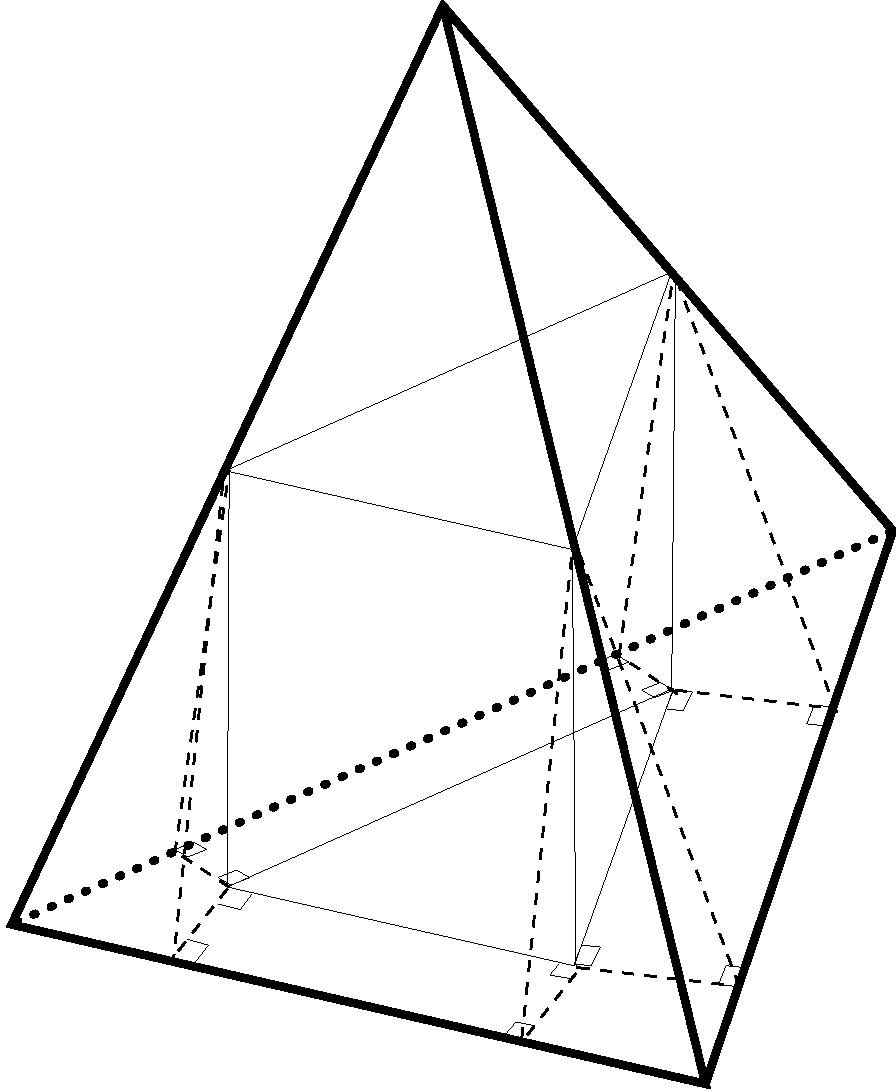
\includegraphics[width=90mm]{figs/pyr.pdf}
%     \end{center}
% \label{pyramid}
% \end{figure}


% Here is an example of using the macros
% \verb2\singlespacing2 and \verb2\doublespacing2:

% \singlespacing	% <------------------------------

% This paragraph was preceded by the
% command \verb2\singlespacing2.
% See the Specifications of the Grad School for instructions
% about when single spacing is appropriate in a thesis.

% \doublespacing	% <------------------------------

% And now, here is an example of using the macros
% \verb2\begin{singlespace}2 and \verb2\end{singlespace}2;
% another way to get single-spacing.

% \begin{singlespace}	% <-----------------------------
% Two cases are studied in the present work which differ only in the
% boundary conditions.  Each different boundary condition model a
% different source of instability.  The boundary of the first case
% consists of a steady, axisymmetric sidewall radial velocity boundary
% and a time-dependent, non-axisymmetric endwall axial velocity
% boundary.  The second case is studied with a fixed impermeable axial
% velocity along the endwall and a combination axisymmetric steady and
% non-axisymmetric unsteady radial velocity along the sidewall.
% \end{singlespace}	% <-----------------------------


% Usually you want to use a table produced by some other
% software, such as Excel, rather than try to do it using
% \LaTeX macros.  If the table is saved/printed to a PDF file,
% then it can be displayed using the
% $\backslash${\tt includegraphics} macro
% inside a {\tt table} environment:


% \begin{table}
%     \caption[Table from a PDF file]{
% 	This table wasn't constructed with \LaTeX{}
% 	commands, but resides in PDF file
% 	({\tt tableD.pdf})
% 	created by some other software.
% 	}
%     \begin{center}
% 	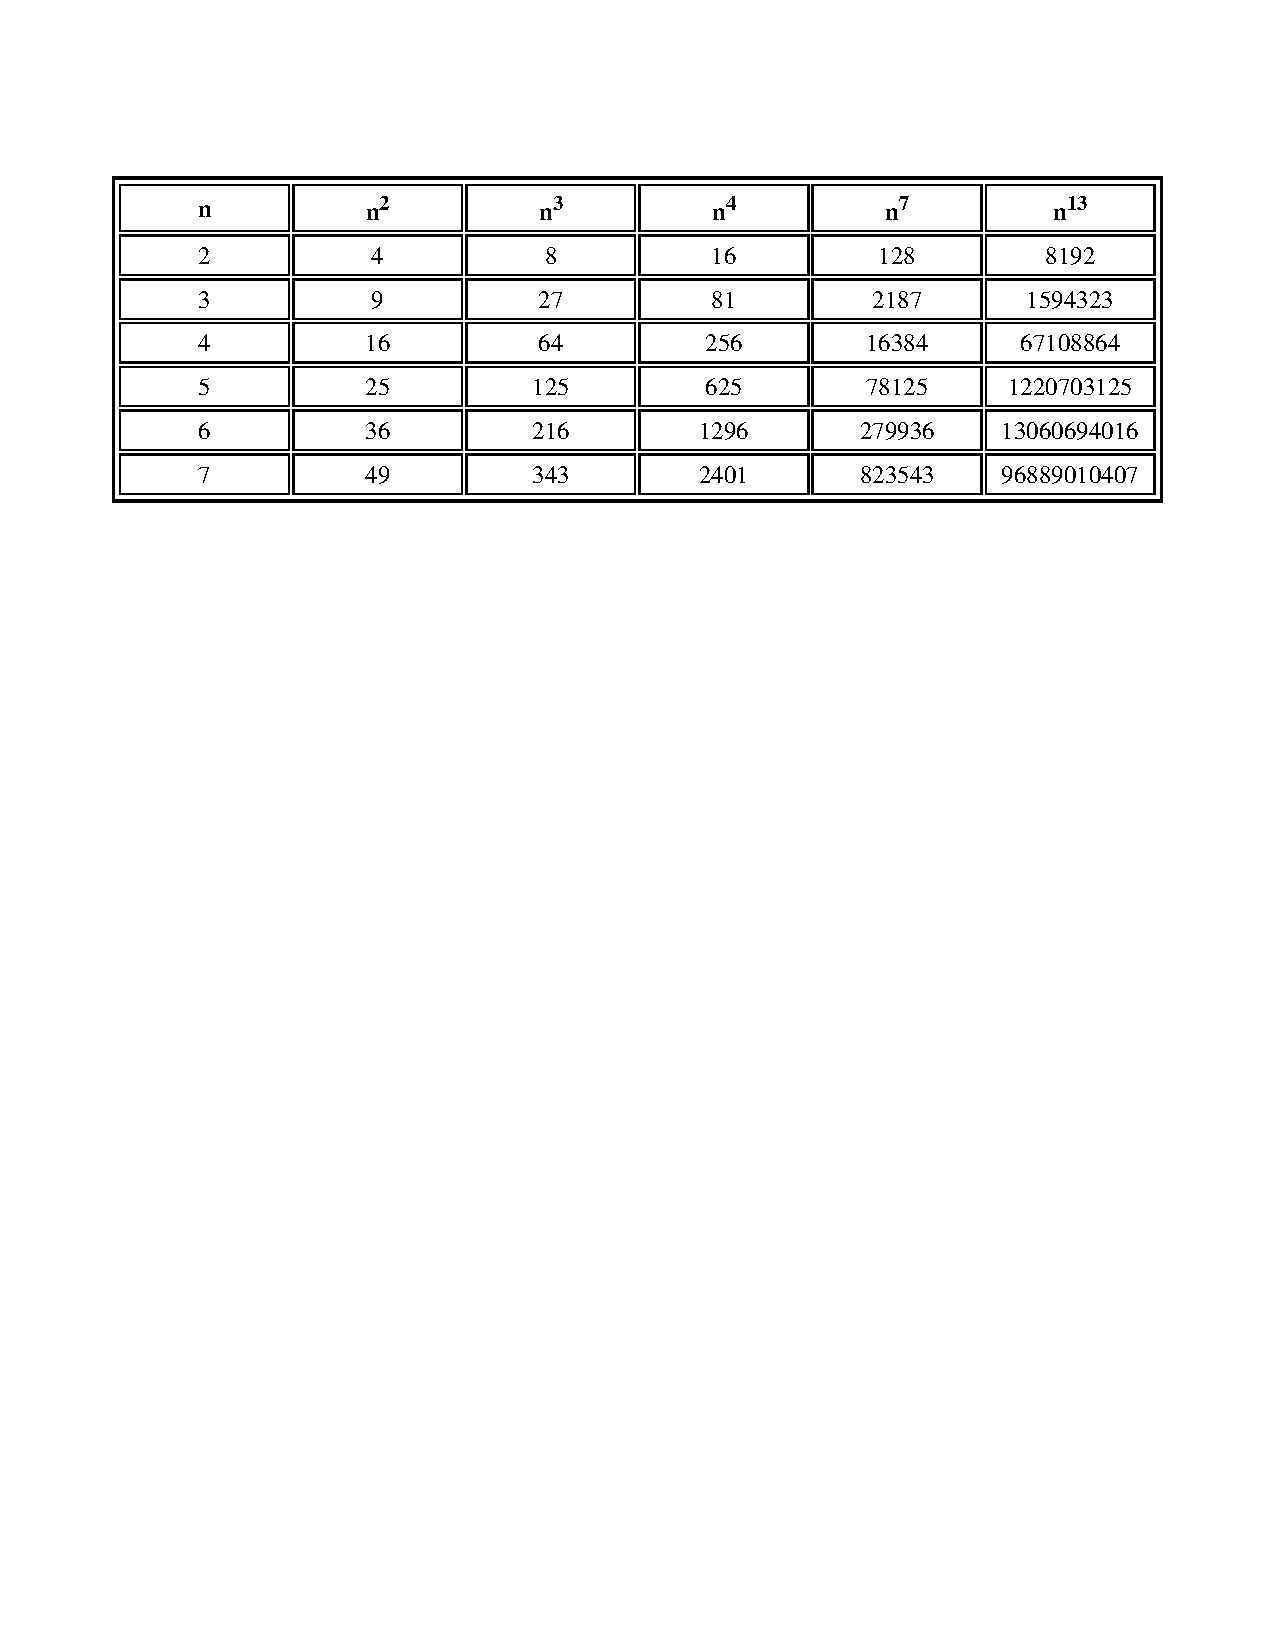
\includegraphics[width=5.45in]{figs/tableD.pdf}
%     \end{center}
% \label{pdftable}
% \end{table}


% Some of the boundary conditions are:

% \begin{eqnarray}
%   z=0; && V_z = \twochoices
% 	{0, && t\leq0}
% 	{\widetilde{F}_{zw}(r,\theta,t), && t>0}
% 						\label{eq:endwall} \\
%   z=0; && V_{\theta}=V_r=0			\label{eq:endnoslip} \\
%   r=0; && P,\rho,T,V_r,\vth,V_z~\mbox{finite},	\label{eq:centerline} \\
%   r=1; && V_r= F_{rws}(z),			\label{eq:injection} \\
%   r=1; && V_z=\vth =0,				\label{eq:sidenoslip}
% \end{eqnarray}
% and solutions must be periodic in $\theta$.

% If you don't believe this stuff, check out
% Mulick\cite{mulick} and Baylor\cite{baylor}.


% \section{Yet another section}

% \subsection{
% 	Just meaningless text to test lines per page
% 	\label{ss}}

% According to the Grad School specs.   there should be 24--27 lines
% of print per page of a thesis.  This should be true whether the font
% size is 10, 11, or 12.  Count them up; does this document conform?
% According to the Grad School specs.   there should be 24--27 lines
% of print per page of a thesis.  This should be true whether the font
% size is 10, 11, or 12.  Count them up; does this document conform?
% According to the Grad School specs.   there should be 24--27 lines
% of print per page of a thesis.  This should be true whether the font
% size is 10, 11, or 12.  Count them up; does this document conform?
% According to the Grad School specs.   there should be 24--27 lines
% of print per page of a thesis.  This should be true whether the font
% size is 10, 11, or 12.  Count them up; does this document conform?
% According to the Grad School specs.   there should be 24--27 lines
% of print per page of a thesis.  This should be true whether the font
% size is 10, 11, or 12.  Count them up; does this document conform?
% According to the Grad School specs.   there should be 24--27 lines
% of print per page of a thesis.  This should be true whether the font
% size is 10, 11, or 12.  Count them up; does this document conform?
% According to the Grad School specs.   there should be 24--27 lines
% of print per page of a thesis.  This should be true whether the font
% size is 10, 11, or 12.  Count them up; does this document conform?
% According to the Grad School specs.   there should be 24--27 lines
% of print per page of a thesis.  This should be true whether the font
% size is 10, 11, or 12.  Count them up; does this document conform?
% According to the Grad School specs.   there should be 24--27 lines
% of print per page of a thesis.  This should be true whether the font
% size is 10, 11, or 12.  Count them up; does this document conform?
% According to the Grad School specs.   there should be 24--27 lines
% of print per page of a thesis.  This should be true whether the font
% size is 10, 11, or 12.  Count them up; does this document conform?
% According to the Grad School specs.   there should be 24--27 lines
% of print per page of a thesis.  This should be true whether the font
% size is 10, 11, or 12.  Count them up; does this document conform?
% According to the Grad School specs.   there should be 24--27 lines
% of print per page of a thesis.  This should be true whether the font
% size is 10, 11, or 12.  Count them up; does this document conform?
% According to the Grad School specs.   there should be 24--27 lines
% of print per page of a thesis.  This should be true whether the font
% size is 10, 11, or 12.  Count them up; does this document conform?
% According to the Grad School specs.   there should be 24--27 lines
% of print per page of a thesis.  This should be true whether the font
% size is 10, 11, or 12.  Count them up; does this document conform?
% According to the Grad School specs.   there should be 24--27 lines
% of print per page of a thesis.  This should be true whether the font
% size is 10, 11, or 12.  Count them up; does this document conform?
% According to the Grad School specs.   there should be 24--27 lines
% of print per page of a thesis.  This should be true whether the font
% size is 10, 11, or 12.  Count them up; does this document conform?
% According to the Grad School specs.   there should be 24--27 lines
% of print per page of a thesis.  This should be true whether the font
% size is 10, 11, or 12.  Count them up; does this document conform?

% \paragraph{What is it?}
% This is a labelled paragraph.
% The heading of the paragraph is emphasized.
% This is a labelled paragraph.
% The heading of the paragraph is emphasized.

% \subsection{This is a subsection}

% This is a subsection.
% Filler filler filler filler filler filler filler filler.
% Filler filler filler filler filler filler filler filler.

% \subsection{This is another subsection}

% This is another subsection.
% Filler filler filler filler filler filler filler filler.
% Filler filler filler filler filler filler filler filler.

% \paragraph{This is paragraph number 2.}
% It used a \verb2\paragraph{}2 header, which
% are always inlined (with extra space)
% and  boldfaced.

% This is the third paragraph of the subsection.
% Filler filler filler filler filler filler filler filler.
% Filler filler filler filler filler filler filler filler.

% %%%%%%%%%%%%%%%%%%%%%%%%%%%%%%%%%%%%%%%%%%%%%%%%%%%%%%%%%%

% \subsubsection{This is a subsubsection (1)}
% This is the first paragraph of the subsubsection.
% Whether it is numbered or inlined depends on the
% option selected at the beginning of the
% thesis.

% By default, a \verb2\subsubsection2 heading is numbered
% and set off on a separate line, left-justified.

% \paragraph{However.}
% Using the \verb2inlineh42 option, subsubsection headers
% are inlined.
% And using the \verb2nonumh42 option suppresses
% numbering of the subsubsections.
% Together they make subsubsection headings
% just the same as paragraph headings.


% %%%%%%%%%%%%%%%%%%%%%%%%%%%%%%%%%%%%%%%%%%%%%%%%%%%%%%%%%%

% \subsubsection{
% 	This is another subsubsection (2)
% 	\label{sss}
% 	}

% Once again, whether its heading is numbered
% and/or inlined depends on the class options
% chosen at the start.

% There is no ``subsubsubsection'' entity,
% and ``subparagraph'' gets no special treatment
% in \emph{thesis} class.

% \section{The End}
% \label{sec:end}

% Finally, this is the end.  The bibliography starts on
% the next page.
% Note how the \verb2\hyperref2 package
% (mentioned in chapter \ref{introchap})
% also makes hyperlinks from references
% (e.g., Mulick\cite{mulick})
% to entries in the bibliography.

